%\renewcommand{\theequation}{\theenumi}
%\begin{enumerate}[label=\arabic*.,ref=\thesubsection.\theenumi]
%\numberwithin{equation}{enumi}
%\item
%
%
%A right angled triangle looks like Fig. \ref{fig:tri_right_angle}.
%\begin{figure}[!ht]
%\centering
%\resizebox{\columnwidth}{!}{%Code by GVV Sharma
%December 6, 2019
%released under GNU GPL
%Drawing a right angled triangle

\begin{tikzpicture}[scale=2]

%Triangle sides
\def\a{4}
\def\c{3}

%Marking coordiantes
\coordinate [label=above:$A$] (A) at (0,\c);
\coordinate [label=left:$B$] (B) at (0,0);
\coordinate [label=right:$C$] (C) at (\a,0);

%Drawing triangle ABC
\draw (A) -- node[left] {$\textrm{c}$} (B) -- node[below] {$\textrm{a}$} (C) -- node[above,,xshift=2mm] {$\textrm{b}$} (A);

%Drawing and marking angles
\tkzMarkAngle[fill=orange!40,size=0.5cm,mark=](A,C,B)
\tkzMarkRightAngle[fill=blue!20,size=.3](A,B,C)
\tkzLabelAngle[pos=0.65](A,C,B){$\theta$}
\end{tikzpicture}
}
%\caption{Right Angled Triangle}
%\label{fig:tri_right_angle}	
%\end{figure}
%with angles $\angle A,\angle B$ and $\angle C$ and sides $a, b$ and $c$.  The unique feature of this triangle is $\angle B$ which is defined to be $90\degree$.
%\item
%	For simplicity, let the greek letter $\theta = \angle C$.  We have the following definitions.
%\begin{equation}
%\label{eq:tri_trig_defs}
%\begin{matrix}
%	\sin \theta = \frac{c}{b} & 	\cos \theta = \frac{a}{b} \\
%	\tan \theta = \frac{c}{a} & \cot \theta = \frac{1}{\tan \theta} \\
%	\csc \theta = \frac{1}{\sin \theta} & \sec \theta = \frac{1}{\cos \theta}
%	\end{matrix}
%\end{equation}
%%
%\item Draw Fig. \ref{fig:tri_right_angle} for $a = 4, c =3$.
%\label{const:tri_right_angle}
%%
%\\
%\solution The vertices of $\triangle ABC$ are 
%\begin{align}
%\vec{A} = \myvec{0\\c} = \myvec{0\\3}, \vec{B} = \myvec{0\\0}, \vec{C} = \myvec{a\\0}=\myvec{4\\0}
%\end{align}
%%
%The python code for  Fig. \ref{fig:tri_right_angle} is
%\begin{lstlisting}
%codes/triangle/tri_right_angle.py
%\end{lstlisting}
%%
%and the equivalent latex-tikz code is
%%
%\begin{lstlisting}
%figs/triangle/tri_right_angle.tex
%\end{lstlisting}
%%
%\item Draw Fig. \ref{fig:tri_polar} for $a = 4, c =3$.
%\label{const:tri_polar}
%%
%\\
%\solution The vertices of $\triangle ABC$ are 
%\begin{align}
%\vec{A} = \myvec{a\\c} = \myvec{4\\3}, \vec{B} = \myvec{a\\0}  = \myvec{4\\0}, \vec{C} = \myvec{0\\0}.
%\end{align}
%%
%The python code for  Fig. \ref{fig:tri_polar} is
%\begin{lstlisting}
%codes/triangle/tri_polar.py
%\end{lstlisting}
%%
%and the equivalent latex-tikz code is
%%
%\begin{lstlisting}
%figs/triangle/tri_polar.tex
%\end{lstlisting}
%\begin{figure}[!ht]
%\centering
%\resizebox{\columnwidth}{!}{%Code by GVV Sharma
%December 6, 2019
%released under GNU GPL
%Drawing a right angled triangle

\begin{tikzpicture}[scale=2]

%Triangle sides
\def\a{4}
\def\c{3}

%Marking coordiantes
\coordinate [label=above:$A$] (A) at (\a,\c);
\coordinate [label=below:$B$] (B) at (\a,0);
\coordinate [label=left:$C$] (C) at (0,0);

%Drawing triangle ABC
\draw (A) -- node[left] {$\textrm{c}$} (B) -- node[below] {$\textrm{a}$} (C) -- node[above left,xshift=2mm] {$\textrm{b}$} (A);

%Drawing and marking angles
\tkzMarkAngle[fill=orange!40,size=0.5cm,mark=](B,C,A)
\tkzMarkRightAngle[fill=blue!20,size=.3](A,B,C)
\tkzLabelAngle[pos=0.65](A,C,B){$\theta$}
\end{tikzpicture}
}
%\caption{Right Angled Triangle}
%\label{fig:tri_polar}	
%\end{figure}
%%
%\item The vertex  $\vec{A}$ can also be expressed  in {\em polar coordinate form} as
%\label{prob:tri_polar}
%%
%\begin{align}
%\vec{A} = \myvec{b\cos \theta\\ b \sin \theta} 
%\end{align}
%%
%
%\end{enumerate}
%
%\subsection{Sum of Angles}
%\renewcommand{\theequation}{\theenumi}
%\begin{enumerate}[label=\arabic*.,ref=\thesubsection.\theenumi]
%\numberwithin{equation}{enumi}
%\item 	In Fig. \ref{fig:tri_sum_angle}, the sum of all the angles on the top or bottom side of the straight line $XY$ is $180\degree$.
%
%
%\begin{figure}[!ht]
%	\begin{center}
%		\resizebox{\columnwidth}{!}{%Code by GVV Sharma
%December 6, 2019
%released under GNU GPL
%Sum of the angles of a right angled triangle 

\begin{tikzpicture}
[scale=2,>=stealth,point/.style={draw,circle,fill = black,inner sep=0.5pt},]

%Triangle sides
\def\a{4}
\def\c{3}

%Section Ratio
\def\k{1.2}


%Labeling points
\node (A) at (0,\c)[point,label=above right:$A$] {};
\node (B) at (0, 0)[point,label=below left:$B$] {};
\node (C) at (\a, 0)[point,label=below right:$C$] {};

%Translating coordinates
\node (Y) at ($(A) + (1,0)$)[point,label=above right:$Y$] {};
\node (X) at ($(A) - (1,0)$)[point,label=above right:$X$] {};
\node (T) at ($(A) + (0,1)$)[point,label=above right:$T$] {};

%Section formula
\node (V) at ($ (C)!\k!(A) $)[point,label=above right:$V$] {};

%Drawing triangle ABC
\draw (A) -- node[left] {$\textrm{c}$} (B) -- node[below] {$\textrm{a}$} (C) -- node[above,xshift=2mm] {$\textrm{b}$} (A);

%Joining other points
\draw (Y)--(A);
\draw (X)--(A);
\draw (T)--(A);
\draw (V)--(A);

%Drawing and marking angles
\tkzMarkAngle[fill=orange!40,size=0.5cm,mark=](A,C,B)
\tkzMarkAngle[fill=orange!40,size=0.5cm,mark=](V,A,X)
\tkzMarkRightAngle[fill=blue!20,size=.3](A,B,C)
\tkzMarkRightAngle[fill=blue!20,size=.3](B,A,X)
\tkzLabelAngle[pos=0.65](A,C,B){$\theta$}
\tkzLabelAngle[pos=0.65](V,A,X){$\theta$}

\end{tikzpicture}
}
%	\end{center}
%	\caption{Sum of angles of a triangle}
%	\label{fig:tri_sum_angle}	
%\end{figure}
%
%
%
%\item
%In Fig. \ref{fig:tri_sum_angle}, the straight line making an angle of $90\degree$ to the side $AB$ is said to be parallel to the side $BC$. Note there is an angle at $A$ that is equal to $\theta$.  This is one property of parallel lines.  Thus, $\angle YAZ = 90\degree$.
%
%
%\item
%	Show that $\angle VAZ = 90\degree - \theta$
%		
%	\solution Considering the line $XAZ$,
%	\begin{align}
%	\theta + 90\degree + \angle VAZ &= 180\degree \\
%	\Rightarrow  \angle VAZ =  90\degree - \theta
%	\end{align}
%
%\item
%	\label{prob:tri_compl_angle}
%	Show that $\angle BAC = 90\degree - \theta$.
%	
%	\solution Consider the line $VAB$ and and use the approach in the previous problem.  Note that this implies that $\angle VAZ = \angle BAC$.  Such angles are known as vertically opposite angles. 
%	 
%\item
%Sum of the angles of a triangle is equal to $180\degree$.
%%
%\item Draw Fig. \ref{fig:tri_sum_angle} for $a = 4, c =3$.
%%
%\\
%\solution Problem \ref{const:tri_right_angle} is used to draw $\triangle ABC$.  The remaining points are obtained as
%
%\begin{align}
%\vec{Y} &= \vec{A} + \myvec{1\\0} = \myvec{1\\3}
%\\
%\vec{X} &= \vec{A} - \myvec{1\\0} = \myvec{-1\\3}
%\\
%\vec{T} &= \vec{A} + \myvec{0\\1} = \myvec{0\\4}
%\end{align}
%%
%and 
%\begin{align}
%\frac{VC}{AC} &= k+1
%\\
%\label{eq:tri_section_formula}
%\implies \vec{A} &= \frac{k\vec{C} + \vec{V}}{k+1}  
%\\
%\implies \vec{V} &= \frac{\brak{k+1}\vec{A} - k\vec{C}}{k}  
%\end{align}
%%
%for $k = 0.2$. \eqref{eq:tri_section_formula} is known as the {\em section formula}.
%%
%The python code for  Fig. \ref{fig:tri_sum_angle} is
%\begin{lstlisting}
%codes/triangle/tri_sum_angle.py
%\end{lstlisting}
%%
%and the equivalent latex-tikz code is
%%
%\begin{lstlisting}
%figs/triangle/tri_sum_angle.tex
%\end{lstlisting}
%\end{enumerate}
%\subsection{Baudhayana Theorem}
%Use Fig. \ref{fig:tri_baudh} for all problems in this section.
%\renewcommand{\theequation}{\theenumi}
%\begin{enumerate}[label=\arabic*.,ref=\thesubsection.\theenumi]
%\numberwithin{equation}{enumi}
%
%
%
%\item  Show that
%	\begin{equation}
%	\cos \theta = \sin \brak{90\degree - \theta}
%	\end{equation}
%
%
%\begin{figure}[!ht]
%	\begin{center}
%		\resizebox{\columnwidth}{!}{%Code by GVV Sharma
%December 7, 2019
%released under GNU GPL
%Proof of Baudhyana Theorem

\begin{tikzpicture}
[scale=2,>=stealth,point/.style={draw,circle,fill = black,inner sep=0.5pt},]

%Triangle sides
\def\a{4}
\def\c{3}
\def\b{sqrt(\a^2+\c^2)}

%Trigonometric ratios
\def\ct{\a/\b}
\def\st{\c/\b}

%perp distance
\def\r{\a*\st}

%Section Ratio
\def\k{1.2}


%Labeling points
\node (A) at (0,\c)[point,label=above right:$A$] {};
\node (B) at (0, 0)[point,label=below left:$B$] {};
\node (C) at (\a, 0)[point,label=below right:$C$] {};

%Foot of perpendicular

\node (D) at ($({\r*\st}, {\r*\ct})$)[point,label=above right:$D$] {};


%Drawing triangle ABC
\draw (A) -- node[left] {$\textrm{c}$} (B) -- node[below] {$\textrm{a}$} (C) -- node[above,xshift=2mm] {$\textrm{b}$} (A);

%Joining BD
\draw (B)--(D);

%Drawing and marking angles
\tkzMarkAngle[fill=orange!40,size=0.5cm,mark=](A,C,B)
\tkzMarkAngle[fill=orange!40,size=0.4cm,mark=](D,B,A)
\tkzMarkAngle[fill=green!40,size=0.5cm,mark=](B,A,C)
\tkzMarkAngle[fill=green!40,size=0.5cm,mark=](C,B,D)
\tkzMarkRightAngle[fill=blue!20,size=.2](A,B,C)
\tkzMarkRightAngle[fill=blue!20,size=.2](B,D,A)
\tkzLabelAngle[pos=0.65](A,C,B){$\theta$}
\tkzLabelAngle[pos=0.65](A,B,D){$\theta$}
\tkzLabelAngle[pos=1](B,A,C){\rotatebox{-45}{$\alpha = 90\degree -\theta$}}
\tkzLabelAngle[pos=0.65](C,B,D){$\alpha$}

\end{tikzpicture}
}
%	\end{center}
%	\caption{Baudhayana Theorem}
%	\label{fig:tri_baudh}	
%\end{figure}
%
%
%\solution From Problem \ref{prob:tri_compl_angle} and  \eqref{eq:tri_trig_defs}
%%
%\begin{multline}
%\label{eq:tri_90-ang}
%\cos \angle BAC = \cos \alpha =	\cos \brak{90\degree-\theta} = \frac{c}{b} 
%\\
%= \sin \angle ABC = \sin \theta
%\end{multline}
%%
%\item
%Show that 
%%
%\begin{equation}
%\label{ch1_budh_basic}
%b = a \cos \theta + c \sin \theta
%\end{equation}
%%
%\solution We observe that
%%
%\begin{align}
%BD &= a \cos \theta \\
%AD &= c \cos\alpha = c \sin \theta \quad \brak{\text{From} \quad \eqref{eq:tri_90-ang}
%}
%\end{align}
%%
%Thus,
%\begin{equation}
%BD + AD = b = a \cos \theta + c \sin \theta
%\end{equation}
%\item
%From \eqref{ch1_budh_basic}, show that
%%
%\begin{equation}
%%
%\label{eq:tri_sin_cos_id}
%\sin ^2 \theta + \cos ^2 \theta = 1
%\end{equation}
%
%
%%
%\solution Dividing both sides of \eqref{ch1_budh_basic} by $b$, 
%\begin{align}
%1 &= \frac{a}{b}\cos\theta + \frac{c}{b}\sin\theta\\
%\Rightarrow &\sin ^2 \theta + \cos ^2 \theta = 1 \quad \brak{\text{from} \quad \eqref{eq:tri_trig_defs}}
%\end{align}
%
%\item
%	Using \eqref{ch1_budh_basic}, show that
%	\begin{equation}
%	\label{eq:tri_baudh}
%	c^2 = a^2 + b^2
%	\end{equation}
%	\eqref{eq:tri_baudh} is known as the Baudhayana theorem.  It is also known as the Pythagoras theorem.
%
%\solution From \eqref{ch1_budh_basic},
%\begin{align}
%c &= a\frac{a}{c} + b \frac{b}{c} \quad \brak{\text{from} \quad \eqref{eq:tri_trig_defs}}\\
%\Rightarrow c^2 &= a^2 + b^2
%\end{align}
%%
%%
%\item Draw Fig. \ref{fig:tri_baudh} for $a = 4, c =3$.
%\label{const:tri_baudh}
%%
%\\
%\solution Problem \ref{const:tri_right_angle} is used to draw $\triangle ABC$.
%%
%Using Problem \ref{prob:tri_polar},
%\begin{align}
%\vec{D} &= BD\myvec{\cos \alpha\\  \sin \alpha} 
%&= a \sin \theta \myvec{ \sin \theta \\ \cos \theta } 
%\label{eq:tri_baudh_foot}
%\end{align}
%%
%Using \eqref{eq:tri_baudh_foot}, the python code for  Fig. \ref{fig:tri_baudh} is
%\begin{lstlisting}
%codes/triangle/tri_baudh.py
%\end{lstlisting}
%%
%and the equivalent latex-tikz code is
%%
%\begin{lstlisting}
%figs/triangle/tri_baudh.tex
%\end{lstlisting}
%%
%\item Using 	\eqref{eq:tri_baudh}, for $a = 4, c = 3$,
%%
%\begin{align}
%b = \sqrt{a^2+c^2} = \sqrt{4^2+3^2} = 5
%\end{align}
%%
%\item For  point $\vec{D} = \myvec{d_1\\d_2}$, its {\em norm} is defined as
%%
%\begin{align}
%OD = d_1^2+d_2^2 = \norm{\vec{D}} \define \sqrt{\vec{D}^T\vec{D}}, 
%\label{eq:tri_norm_def}
%\end{align}
%%
%where 
%%
%\begin{align}
%\label{eq:tri_transpose_def}
% \vec{D}^T  \define \myvec{d_1 & d_2},
%\\
%\vec{D}^T\vec{D} \define \myvec{d_1 & d_2} \myvec{d_1 \\ d_2} = d_1^2+d_2^2
%\end{align}
%%
%\eqref{eq:tri_transpose_def} is the definition of {\em transpose}. $\vec{D}$ is defined to be a {\em column vector} and $\vec{D}^T$  is the corresponding {\em row vector} representing the same point.
%
%\item Also, it is easy to verify that
%%
%\begin{align}
%\label{eq:tri_norm_dist}
%AC \define  \norm{\vec{A}-\vec{C}} =  \norm{\myvec{4\\-3}} = \sqrt{3^2+4^2} = 5
%\end{align}
%%
%This is known as the {\em distance formula}.
%%
%\item Prove the distance formula in \eqref{eq:tri_norm_dist} using Baudhayana theorem.
%
%\end{enumerate}
\renewcommand{\theequation}{\theenumi}
\begin{enumerate}[label=\arabic*.,ref=\thesubsection.\theenumi]
\numberwithin{equation}{enumi}
%



\item
	The area of the rectangle $ACBD$ shown in Fig. \ref{fig:tri_rect} is defined as $ac$. Note that all the angles in the rectangle are $90\degree$
%	\label{fig:tri_rect}

\begin{figure}[!ht]
	\begin{center}
		
		%\includegraphics[width=\columnwidth]{./figs/fig:tri_rect}
		%\vspace*{-10cm}
		\resizebox{\columnwidth}{!}{%Code by GVV Sharma
%December 7, 2019
%released under GNU GPL
%Drawing a rectangle

\begin{tikzpicture}
[scale=2,>=stealth,point/.style={draw,circle,fill = black,inner sep=0.5pt},]

%Triangle sides
\def\a{4}
\def\c{3}

%Marking coordiantes
\coordinate [label=above:$A$] (A) at (0,\c);
\coordinate [label=left:$B$] (B) at (0,0);
\coordinate [label=right:$C$] (C) at (\a,0);

%Drawing triangle ABC
\draw (A) -- node[left] {$\textrm{c}$} (B) -- node[below] {$\textrm{a}$} (C) -- node[above,,xshift=2mm] {$\textrm{b}$} (A);

\node (D) at (\a, \c)[point,label=above right:$D$] {};

%Joining AD and CD
\draw (A)--(D);
\draw (C)--(D);

%Drawing and marking angles
\tkzMarkRightAngle[fill=blue!20,size=.3](A,B,C)
\tkzMarkRightAngle[fill=blue!20,size=.3](A,D,C)
\end{tikzpicture}
}
	\end{center}
	\caption{Area of a Right Triangle}
	\label{fig:tri_rect}	
\end{figure}
%
\item Draw Fig. \ref{fig:tri_rect} for $a = 4, c =3$.
\label{const:tri_rect}
\\
\solution Letting
%
\begin{align}
\vec{B} = \myvec{0 \\  0}, 
\vec{D} = \myvec{4 \\  3} 
\label{eq:tri_rect}
\end{align}
%
the python code for  Fig. \ref{fig:tri_rect} is
\begin{lstlisting}
codes/triangle/tri_rect.py
\end{lstlisting}
%
and the equivalent latex-tikz code is
%
\begin{lstlisting}
figs/triangle/tri_rect.tex
\end{lstlisting}

\item
	The area of the two triangles constituting the rectangle is the same.
	\label{ch2_triang_eq}

\item
	The area of the rectangle is the sum of the areas of the two triangles inside.
	\label{ch2_triang_sum}


\item
\label{prob:ch2_triang_area}
	Show that the area of $\Delta ABC$ is $\frac{ac}{2}$

\begin{figure}[!ht]
	\begin{center}
		
		%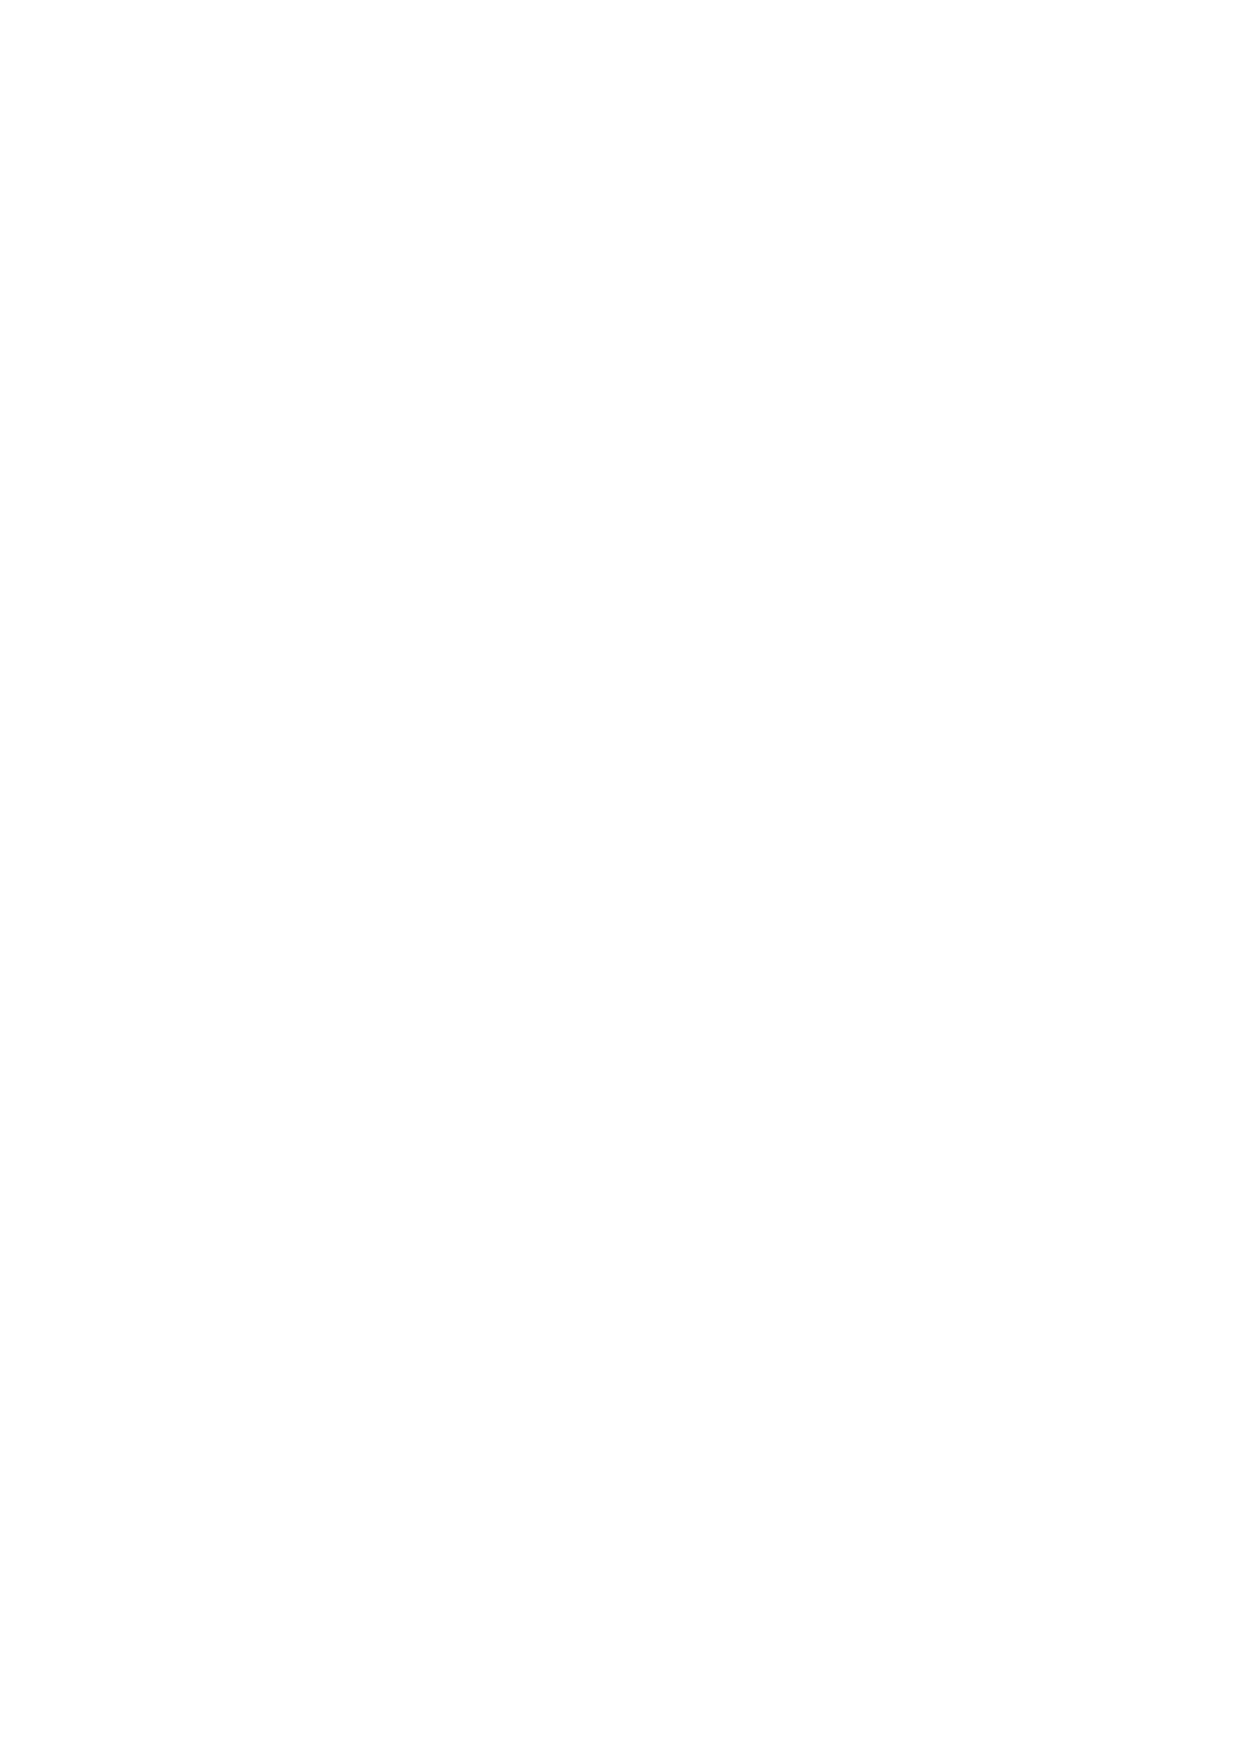
\includegraphics[width=\columnwidth]{./figs/ch2_triang_ar}
		%\vspace*{-10cm}
		\resizebox{\columnwidth}{!}{%Code by GVV Sharma
%December 7, 2019
%released under GNU GPL
%Drawing a triangle given 3 sides

\begin{tikzpicture}
[scale=2,>=stealth,point/.style={draw,circle,fill = black,inner sep=0.5pt},]

%Triangle sides
\def\a{6}
\def\b{5}
\def\c{4}
 
%Coordinates of A
%\def\p{{\a^2+\c^2-\b^2}/{(2*\a)}}
\def\p{2.25}
\def\q{{sqrt(\c^2-\p^2)}}

%Labeling points
\node (A) at (\p,\q)[point,label=above right:$A$] {};
\node (B) at (0, 0)[point,label=below left:$B$] {};
\node (C) at (\a, 0)[point,label=below right:$C$] {};

%Foot of perpendicular

\node (D) at (\p,0)[point,label=above right:$D$] {};

%Drawing triangle ABC
\draw (A) -- node[left] {$\textrm{c}$} (B) -- node[below] {$\textrm{a}$} (C) -- node[above,xshift=2mm] {$\textrm{b}$} (A);

%Drawing altitude AD
\draw (A) -- node[left] {$\textrm{h}$}(D);

%Drawing and marking angles
%\tkzMarkAngle[fill=orange!40,size=0.5cm,mark=](A,C,B)
%\tkzMarkAngle[fill=orange!40,size=0.4cm,mark=](D,B,A)
%\tkzMarkAngle[fill=green!40,size=0.5cm,mark=](B,A,C)
%\tkzMarkAngle[fill=green!40,size=0.5cm,mark=](C,B,D)
\tkzMarkRightAngle[fill=blue!20,size=.2](A,D,B)
%\tkzMarkRightAngle[fill=blue!20,size=.2](B,D,A)
%\tkzLabelAngle[pos=0.65](A,C,B){$\theta$}
%\tkzLabelAngle[pos=0.65](A,B,D){$\theta$}
%\tkzLabelAngle[pos=1](B,A,C){\rotatebox{-45}{$\alpha = 90\degree -\theta$}}
%\tkzLabelAngle[pos=0.65](C,B,D){$\alpha$}

\end{tikzpicture}
}
	\end{center}
	\caption{Area of a Triangle}
	\label{fig:tri_sss}	
\end{figure}

\solution From\eqref{ch2_triang_sum},
\begin{equation}
\label{ch2_triang_ar_1}
ar\brak{ABCD} = ar\brak{ACB} + ar\brak{ADB}
\end{equation}
Also from \eqref{ch2_triang_eq},
\begin{equation}
\label{ch2_triang_ar_2}
ar\brak{ACB} = ar\brak{ADB}
\end{equation}
From \eqref{ch2_triang_ar_1} and \eqref{ch2_triang_ar_2},
\begin{align}
2ar\brak{ACB} &= ar\brak{ABCD} = ac \brak{\text{from} \quad \eqref{fig:tri_rect}}
\\
\Rightarrow ar\brak{ACB} &= \frac{ac}{2}
\end{align}

\item
	Show that the area of $\Delta ABC$ in Fig. 	\ref{fig:tri_sss}	is $\frac{1}{2}ah$.


\solution In Fig. \ref{fig:tri_sss},
\begin{align}
ar\brak{\Delta ADC} &= \frac{1}{2}hy \\
ar\brak{\Delta ADB} &= \frac{1}{2}hx 
\end{align}
Thus,
\begin{align}
ar\brak{\Delta ABC} &= ar\brak{\Delta ADC} + ar\brak{\Delta ADB} \\
&= \frac{1}{2}hy + \frac{1}{2}hx = \frac{1}{2}h\brak{x+y} \\
&= \frac{1}{2}ah
\end{align}
%
\item Draw Fig. \ref{fig:tri_sss} with $a=6$, $b=5$  and $c=4$.  
\label{const:tri_sss}
\\
\solution Let the vertices of  $\triangle ABC$ and $\vec{D}$ be 
\begin{align}
\label{eq:tri_basic}
\vec{A} = \myvec{p\\q}, \vec{B} = \myvec{0\\0}, \vec{C} = \myvec{a\\0}, \vec{D} = \myvec{p\\0}
\end{align}
%

Then
\begin{align}
\label{eq:c_tricoord}
AB &= \norm{\vec{A}-\vec{B}}^2 = \norm{\vec{A}}^2  = c^2 \quad \because \vec{B} = \vec{0}
\\
\label{eq:a_tricoord}
BC &= \norm{\vec{C}-\vec{B}}^2 = \norm{\vec{C}}^2  = a^2
\\
AC &= \norm{\vec{A}-\vec{C}}^2 =    b^2
\label{eq:b_tricoord}
\end{align}
%
From \eqref{eq:b_tricoord},
\begin{align}
b^2 &=\norm{\vec{A}-\vec{C}}^2 = \norm{\vec{A}-\vec{C}}^T\norm{\vec{A}-\vec{C}}  
\\
&= \vec{A}^T\vec{A}+\vec{C}^T\vec{C}-\vec{A}^T\vec{C} - \vec{C}^T\vec{A} 
\\
&= \norm{\vec{A}}^2 + \norm{\vec{C}}^2 - 2\vec{A}^T\vec{C} \quad \brak{\because \vec{A}^T\vec{C} = \vec{C}^T\vec{A} } 
\label{eq:tri_const_norm_ac}
\\
&= a^2+c^2-2ap
\end{align}
%
yielding
\begin{align}
p&= \frac{a^2+c^2-b^2}{2a}
\end{align}
%
From \eqref{eq:c_tricoord}, 
\begin{align}
\norm{\vec{A}}^2 &= c^2 = p^2+q^2
\\
\implies q&= \pm \sqrt{c^2-p^2}
\end{align}
%
The python code for  Fig. \ref{fig:tri_sss} is
\begin{lstlisting}
codes/triangle/tri_sss.py
\end{lstlisting}
%
and the equivalent latex-tikz code is
%
\begin{lstlisting}
figs/triangle/tri_sss.tex
\end{lstlisting}

\item
\label{prob:tri_area_sin}
	Show that the area of $\Delta ABC$ in Fig. 	\ref{fig:tri_sss}	is $\frac{1}{2}ab \sin C$.

\solution We have
%
\begin{equation}
ar\brak{\Delta ABC} = \frac{1}{2}ah = \frac{1}{2}ab\sin C \quad \brak{\because \quad h = b \sin C}.
\end{equation}
%
\item
	Show that 
	\begin{equation}
	\frac{\sin A}{a} = \frac{\sin B}{b} = \frac{\sin C}{c}
	\end{equation}

\solution Fig. \ref{fig:tri_sss} can be suitably modified to obtain 
\begin{equation}
ar\brak{\Delta ABC} = \frac{1}{2}ab\sin C = \frac{1}{s}bc\sin A = \frac{1}{2}ca\sin B
\end{equation}
Dividing the above by $abc$, we obtain
	\begin{equation}
\label{eq:tri_sin_form}
	\frac{\sin A}{a} = \frac{\sin B}{b} = \frac{\sin C}{c}
	\end{equation}
This is known as the sine formula.	
%
\item
In Fig. \ref{fig:tri_cosine_formula}, show that
%
\begin{equation}
\label{eq:tri_cos_form}
\cos A = \frac{b^2+c^2-a^2}{2bc}
\end{equation}
%
\

\begin{figure}[!ht]
	\begin{center}
		
		%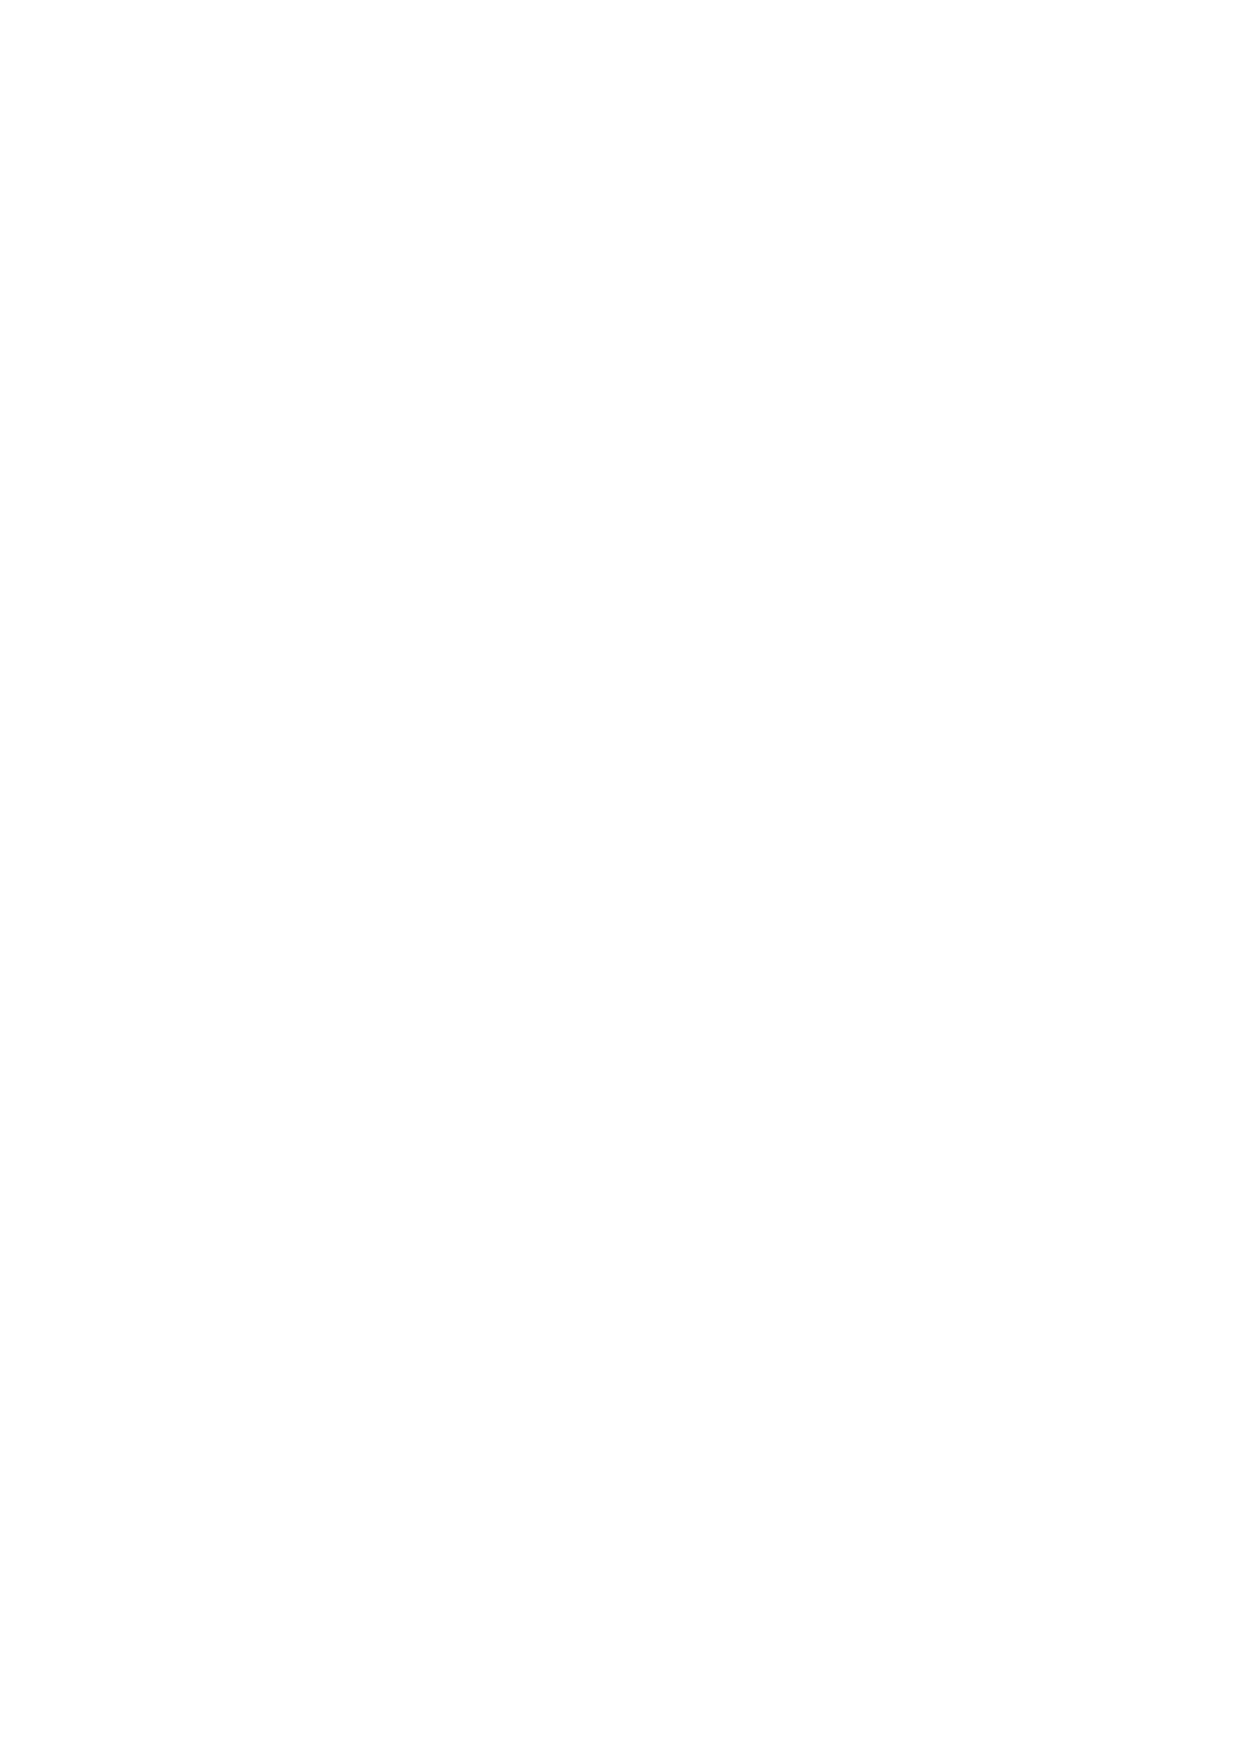
\includegraphics[width=\columnwidth]{./figs/ch2_triang_ar}
		%\vspace*{-10cm}
		\resizebox{\columnwidth}{!}{%Code by GVV Sharma
%December 7, 2019
%released under GNU GPL
%Drawing a triangle given 3 sides

\begin{tikzpicture}
[scale=2,>=stealth,point/.style={draw,circle,fill = black,inner sep=0.5pt},]

%Triangle sides
\def\a{6}
\def\b{5}
\def\c{4}
 
%Coordinates of A
%\def\p{{\a^2+\c^2-\b^2}/{(2*\a)}}
\def\p{2.25}
\def\q{{sqrt(\c^2-\p^2)}}

%Labeling points
\node (A) at (\p,\q)[point,label=above right:$A$] {};
\node (B) at (0, 0)[point,label=below left:$B$] {};
\node (C) at (\a, 0)[point,label=below right:$C$] {};

%Foot of perpendicular

\node (D) at (\p,0)[point,label=above right:$D$] {};

%Drawing triangle ABC
\draw (A) -- node[left] {$\textrm{c}$} (B) -- node[below] {$\textrm{a}$} (C) -- node[above,xshift=2mm] {$\textrm{b}$} (A);

%Drawing altitude AD
\draw (A) -- node[left] {$\textrm{h}$}(D);

\tkzMarkRightAngle[fill=blue!20,size=.2](A,D,B)

\node [below] at ($(B)!0.5!(D)$) {$x$};
\node [below] at ($(C)!0.5!(D)$) {$y$};

\end{tikzpicture}
}
	\end{center}
	\caption{The cosine formula}
	\label{fig:tri_cosine_formula}	
\end{figure}

\solution From the figure, the first of the following equations
%
\begin{align}
a &= b \cos C + c \cos B \\
b &= c \cos A + a \cos C \\
c &= b \cos A + a \cos B
\end{align}
%
is obvious and the other two can be similarly obtained.  The above equations can be expressed in matrix form as
%
\begin{equation}
\begin{pmatrix}
0 & c & b \\
c & 0 & a \\
b & a & 0
\end{pmatrix}
\begin{pmatrix}
\cos A \\
\cos B \\
\cos C
\end{pmatrix}
= 
\begin{pmatrix}
a\\
b\\
c
\end{pmatrix}
\end{equation}
%
Using the properties of determinants,
%
\begin{align}
\cos A &= \frac{
\begin{vmatrix}
a & c & b \\
b & 0 & a \\
c & a & 0
\end{vmatrix}
	}
	{
\begin{vmatrix}
0 & c & b \\
c & 0 & a \\
b & a & 0
\end{vmatrix}
	}
	=\frac{ab^2 + ac^2 - a^3}{abc + abc} 
\\
&= \frac{b^2 + c^2 - a^2}{2abc}
\end{align}
%
\item Find Hero's formula for the area of a triangle.
\\
\solution 
%In Fig. \ref{fig:rt_triangle}, from Baudhayana's theorem, 
%\begin{align}
%\label{eq:tri_geo_baudh}
%b^2 = a^2+c^2 &
%\\
%=b^2\cos^2C+b^2\sin^2C &
%\\
%\implies \cos^2C+\sin^2C &= 1
%\end{align}
%
%In Fig. \ref{fig:tri_const_ex_cos_form}, 
From \eqref{prob:tri_area_sin}, the area of $\triangle ABC$ is 
{\footnotesize
\begin{align}
\label{eq:tri_geo_area_sin_form}
 \frac{1}{2}ab\sin C
%\\
&=\frac{1}{2}ab\sqrt{1-\cos^2C} 
\quad \brak{\text{from } \eqref{eq:tri_sin_cos_id}
%\eqref{eq:tri_geo_baudh}
}
\\
&=\frac{1}{2}ab\sqrt{1-\brak{\frac{a^2+b^2-c^2}{2ab}}^2} \brak{\text{from } \eqref{eq:tri_cos_form}
}
\\
&=\frac{1}{4}\sqrt{\brak{2ab}^2-\brak{a^2+b^2-c^2}}
\\
&=\frac{1}{4}\sqrt{\brak{2ab+a^2+b^2-c^2}\brak{2ab-a^2-b^2+c^2}}
\\
&= \frac{1}{4}\sqrt{\cbrak{\brak{a+b}^2-c^2}\cbrak{c^2-\brak{a-b}^2}}
\\
&= \frac{1}{4}\sqrt{\brak{a+b+c}\brak{a+b-c}\brak{a+c-b}\brak{b+c-a}}
\label{eq:tri_ex_hero_temp}
\end{align}
}
Substituting 
%
\begin{align}
s=\frac{a+b+c}{2}
\end{align}
%
in \eqref{eq:tri_ex_hero_temp}, the area of $\triangle ABC$ is 
%
\begin{align}
\label{eq:tri_hero}
\sqrt{s\brak{s-a}\brak{s-b}\brak{s-c}}
\end{align}
%
This is known as Hero's formula.
\end{enumerate}


